
\noindent \textbf{L3.2 (Sipser 1.49)} Reescrevi o enunciado substituindo $y$ por $w$ para não confundir com as propriedades do lema do bombeamento. Para ambas as questões o alfabeto é $\Sigma = \{0, 1\}$.

\begin{enumerate}[label={\textbf{\alph*.}}]
    \item Seja $B = \{1^kw \ |\ w\ \in \Sigma^*$ e $w$ contém pelo menos $k$ 1s, para $k \geq 1\}$.\\
    Mostre que $B$ é uma linguagem regular.
    
    \textbf{Resposta:} Se $B$ é uma linguagem regular, então existe um autômato finito que a reconhece.
    
    Podemos observar algumas cadeias que pertencem a $B$, tais como, $111|00111$, $1|10$, $1|11$, $1|01$ e outras que não pertencem a $B$, tais como, $0|0$, $0|1$, $1|00$, onde $|$ indica o final da subcadeia $1^k$. Percebemos, então, que as cadeias em $B$ não podem começar com 0 e, as que estão em $B$ devem, necessariamente, começar em 1, já que $k \geq 1$.
    
    Logo, podemos reescrever $B$ como $B = \{1x \ |\ x \in \Sigma^*$ e $x$ tem pelo menos um 1$\}$.
    
    Agora, vamos construir um AFD $M = (Q, \Sigma, \delta, s, F)$ que reconhece $B$:
    \begin{center}
    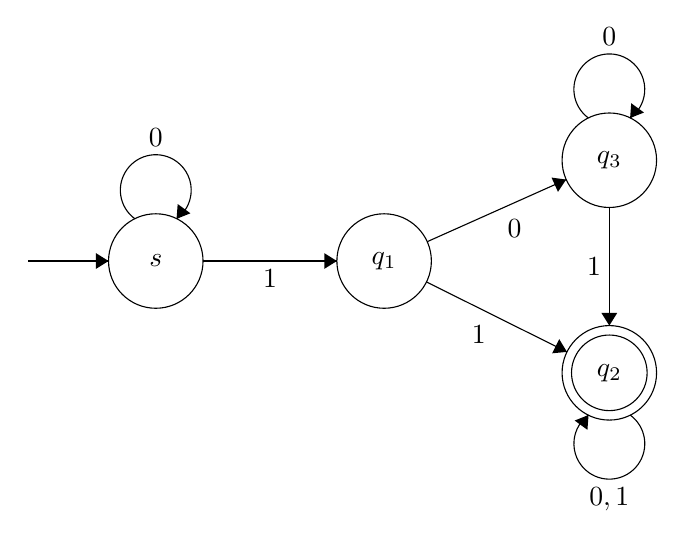
\begin{tikzpicture}[scale=0.2]
    \tikzstyle{every node}+=[inner sep=0pt]
    \draw [black] (17.6,-24.8) circle (3);
    \draw (17.6,-24.8) node {$s$};
    \draw [black] (32.1,-24.8) circle (3);
    \draw (32.1,-24.8) node {$q_1$};
    \draw [black] (46.4,-18.4) circle (3);
    \draw (46.4,-18.4) node {$q_3$};
    \draw [black] (46.4,-31.9) circle (3);
    \draw (46.4,-31.9) node {$q_2$};
    \draw [black] (46.4,-31.9) circle (2.4);
    \draw [black] (9.5,-24.8) -- (14.6,-24.8);
    \fill [black] (14.6,-24.8) -- (13.8,-24.3) -- (13.8,-25.3);
    \draw [black] (16.277,-22.12) arc (234:-54:2.25);
    \draw (17.6,-17.55) node [above] {$0$};
    \fill [black] (18.92,-22.12) -- (19.8,-21.77) -- (18.99,-21.18);
    \draw [black] (20.6,-24.8) -- (29.1,-24.8);
    \fill [black] (29.1,-24.8) -- (28.3,-24.3) -- (28.3,-25.3);
    \draw (24.85,-25.3) node [below] {$1$};
    \draw [black] (34.84,-23.57) -- (43.66,-19.63);
    \fill [black] (43.66,-19.63) -- (42.73,-19.5) -- (43.14,-20.41);
    \draw (40.38,-22.11) node [below] {$0$};
    \draw [black] (34.79,-26.13) -- (43.71,-30.57);
    \fill [black] (43.71,-30.57) -- (43.22,-29.76) -- (42.77,-30.66);
    \draw (38.11,-28.86) node [below] {$1$};
    \draw [black] (46.4,-21.4) -- (46.4,-28.9);
    \fill [black] (46.4,-28.9) -- (46.9,-28.1) -- (45.9,-28.1);
    \draw (45.9,-25.15) node [left] {$1$};
    \draw [black] (45.077,-15.72) arc (234:-54:2.25);
    \draw (46.4,-11.15) node [above] {$0$};
    \fill [black] (47.72,-15.72) -- (48.6,-15.37) -- (47.79,-14.78);
    \draw [black] (47.723,-34.58) arc (54:-234:2.25);
    \draw (46.4,-39.15) node [below] {$0,1$};
    \fill [black] (45.08,-34.58) -- (44.2,-34.93) -- (45.01,-35.52);
    \end{tikzpicture}
    \end{center}
    

    \item Seja $C = \{1^kw \ |\ w\ \in \Sigma^*$ e $w$ contém no máximo $k$ 1s, para $k \geq 1\}$.\\
    Mostre que $C$ nâo é uma linguagem regular.
    
    \textbf{Resposta:} Vamos usar o lema do bombeamento para mostrar que $C$ não é regular. A prova é por contradição.
    
    Suponha o contrário, ou seja, que $C$ é regular. Seja $p$ o comprimento de bombeamento dado pelo lema do bombeamento. Seja $s$ a cadeia $s = 1^p01^p$. Como $s \in C$ e $|s| \geq p$, o lema do bombeamento garante que $s$ pode ser dividida em três partes $s = xyz$ com $x = 1^a$, $y = 1^b$ e $z = 1^c01^p$, onde, $b \geq 1$ e $a + b + c = p$. Vamos mostrar que isso é impossível.
    
    Vamos tomar a cadeia $s' = xy^0z = 1^{a+c}01^p$. Como $b \geq 1$ e $a + b + c = p$, nós temos que $a + c < p$ e, sendo assim, $s' \notin C$, o que contradiz a condição 1 do lema do bombeamento.
    
    Portanto, podemos concluir que $C$ não é regular.
\end{enumerate}